\documentclass[submit]{aiaa-pretty-modified}

\usepackage{graphicx}
\usepackage{array}
\usepackage{amsmath}
\usepackage{amssymb}
\usepackage{multirow}
\usepackage{rotating}
\usepackage[header,page]{appendix}
\usepackage{placeins}
\usepackage{pdfpages}

\title{\textbf{Planning Algorithms for Indoor Robotic Odor Localization}
\\  16.622 Final Report}

\date{\today}

\author{Authors: \\Troy Astorino \\ Mark Van de Loo \\
  \\ 
  Advisors:\\ Professor Youssef Marzouk \\ Professor Nicholas
    Roy \\ Josh Joseph \\ Javier Velez \\ Xun Huan \\ Sachi Hemachandra}

\newcommand{\tablewidth}[0]{1in}
\newcommand{\tablewidthtwo}[0]{3in}
\newcount\colveccount
\newcommand*\colvec[1]{
  \global\colveccount#1
  \begin{pmatrix}
    \colvecnext
  }
  \def\colvecnext#1{
    #1
    \global\advance\colveccount-1
    \ifnum\colveccount>0
    \\
    \expandafter\colvecnext
    \else
  \end{pmatrix}
  \fi
}

\begin{document}
\maketitle

\newpage

\tableofcontents

\newpage

\section{Introduction}

Odor localization is defined as ``the act of finding the location of a
volatile chemical source in the environment.''\cite{kowadlo} Odor
localization is an essential process for many biological systems, from
moths following pheromone trails to find mates, to bacteria finding a
food source. The field of robotic odor localization, which has drawn
much inspiration from biological processes, promises many benefits to
humanity today. Robots could use odor localization to accomplish tasks
in environments that would prove dangerous for humans: finding the
source of toxic chemical leaks for instance, or finding people
trapped in a collapsed building or mine.

There has been little robotic odor localization research done in indoor
environments. This is due to the difficulty of modeling turbulence in a typical
room. Accurate prediction of airflow requires precise knowledge of the geometry
and ventilation of the room, and even if these are known, prediction is too
computationally expensive to perform in real-time on a robot. Instead of trying
to precisely predict how airflows affect indoor vapor dispersion, this
experiment will attempt to use localization algorithms robust enough to overcome
transient turbulence introduced by indoor air currents. Our experiment will
address the problem of odor localization in irregularly shaped rooms through the
use of gradient descent approaches to autonomous path planning.

\section{Hypothesis, Objective, Success Criteria}
\label{sec:hos}
\subsection*{Hypothesis} 
The mean localization rate of a 45-minute two-dimensional search by an
autonomous ground robot equipped with a chemical vapor sensor will be
20 percent greater using a stochastic planner than using a simple gradient descent planner.
\footnote{
  A simple gradient descent algorithm will
  take samples from regions neighboring the robot’s current location, 
  and will always move in the direction of the neighboring region with
  the strongest reading. A stochastic algorithm will add some randomness
  to the choice of the next location the robot will move towards,
  allowing the planning algorithm to gain a more complete representation
  of the search space, at the potential cost of taking some unnecessary
  measurements.}

\subsection*{Objective}
Equip a ground robot furnished by the CSAIL Robust Robotics Group with an Alpha MOS NEEM chemical sensor, implement the planners on the robot’s software platform, and assess the mean localization rate of a cup of ethanol in a closed room.

\subsection*{Success Criteria} 
Determine the difference in mean localization rate to a sufficient precision such that the hypothesis can be assessed.

\section{Literature Review}
Approaches to robotic odor localization may be analyzed as a combination of
three components: a model, an estimator, and a planner. The model is a
mathematical function that describes the spatiotemporal variation of the
chemical concentration. The estimator represents the process by which
measurements of the chemical concentration are combined with model in real time
to obtain an estimate of the location of the chemical source. The planner is an
algorithm that decides the location of the next measurement given the current
estimate and confidence interval of the source location.

Review of previous work in the field of robot odor localization helped to select
this experiment’s test environment of windless indoor rooms with uncommon
geometries. In addition, it provided the basis for the selection of a Bayesian inference
estimator and a Gaussian model to be selected as parameters of the experiment, and
motivated the selection of a simple gradient descent planner and a stochastic
gradient descent planner as interchangeable parts of the localization algorithm
to be compared for speed.

\subsection{Experiment Motivation}
Robotic odor localization experiments have been conducted using chemical
dispersion in water, air, and soil.\cite{kowadlo} In water and soil, diffusion is the
dominating method by which a chemical emanates from a source and disperses
through space. In air, where the Reynolds number is higher than in water or
soil, the behavior of the chemical concentration is affected by the presence of
turbulent fluid currents in addition to chemical diffusion.\cite{kowadlo} These turbulent
currents have led most robotic odor localization researchers to introduce an
artificial wind source when working in air. This negates the effect of the
turbulence, producing a concentration plume that behaves as a 2-dimensional
Gaussian function in planes normal to the wind direction, and downwind of the
source. \cite{ferri} While smoothing the concentration field in this manner makes the task of locating the
chemical source more straightforward, this environment is not representative of
a realistic indoor scenario. A few experiments, such as that done by Ferri, et
al., have been conducted in an indoor environment without an artificial wind
source. \cite{ferri} In general, however, it seems that turbulent indoor environments
have been less explored than their artificial wind source counterparts. For this
reason, it was decided that this experiment will be conducted in an ambient,
windless indoor environment. In addition, the experiment will attempt robot odor
localization in test rooms with floor plans that are not rectangular and have
non-intuitive geometries, which to the knowledge of the authors has not been done
previously.

\subsection{Selection of Model and Estimator}
Due to the varying effects of turbulence and diffusion discussed in section 3.1,
accurate modeling of the concentration field is dependent upon the medium and
environment in which the experiment is conducted. However, many robotic odor
localization researchers chose not to use a high-fidelity model of the
concentration field, deeming this level of complexity unnecessary. \cite{kowadlo} Most
commonly used was a dispersion model based on a Gaussian function. Time
invariant Gaussian models were used successfully in experiments in water and
soil, as well as in air with an artificial wind source. \cite{kowadlo} In turbulent air,
Ferri, et al. successfully used a time invariant monotonic function with a
single peak at the source location as a concentration model. \cite{ferri} The two
algorithms tested both successfully localized a dish of ethanol in a mean time
of less than 10 minutes, beginning an average distance of 1.8m from the source.
The model used in these localization algorithms is not explicitly described in
\cite{ferri}, but the assumption that the model is time invariant and monotonic with a
single peak is a defining component of the successful localization algorithms
presented in this paper. Based on the success of Ferri, et al., it was decided
that this experiment would use a Gaussian concentration field model, treating
the effects of turbulent fluid currents in the air as noise. A Bayesian filter
was selected as an estimator to account for this noise in determining a
probability distribution of the source location after each measurement. The
Bayesian filter is a common technique used in conjunction with Gaussian models
in robotic localization and is described in \cite{bergman}.

\subsection{Selection of Planners}
Planners that were shown to be effective in turbulent air environments were
mainly derived from observations of the behavior of biological organisms.
\cite{ferri} For example, Ferri et al. attempted to mimic the circling behavior
of the Luna Moth in its search for a mate in one planner, and the weighted
random walk exhibited by the chemotaxis3 of the E. coli bacterium in another.
\cite{ferri} No documentation of simple gradient descent using a single sensor
or other simple statistically motivated planners as applied to robot odor
localization was found. Using simple gradient descent is attractive because of
its simplicity, but due to the turbulent nature of ambient indoor air, a simple
gradient descent planner may be prone to confusion by temporary local maxima of
the chemical concentration. An alternative planner that may perform better in
the turbulent environment without requiring a complicated model is based on
stochastic gradient descent, which adds randomness to the gradient vector when
prescribing the direction of motion. \cite{bottou} This randomness helps avoid
the issues caused by temporary local maxima.

\section{Description of Experiment}
\subsection{Experimental Overview}
In this experiment two different planning algorithms will be tested using the
same model and estimation method. A sensor capable of identifying the
concentration of ethanol in the surrounding air will be mounted on a ground
robot. The mean time the robot takes to localize the ethanol source using a
stochastic gradient descent planning algorithm will be compared to the mean time
taken using a simple gradient descent planning algorithm.

\subsection{Test Apparatus}
\label{sec:design}
\subsubsection{Robot Hardware}

An Alpha MOS NEEM chemical sensor (Figure~\ref{fig:sensor}) will be attached to
the mounting pole of the Envoy robotic platform of the Robust Robotics Group.
The robot and the mounting pole can be seen in Figure~\ref{fig:wheelchair}. All
data processing will occur on a laptop mounted on the robot. The laptop will
also be responsible for motion commands and navigation.

\begin{figure}
\begin{center}
\includegraphics[width=5in]{img/wheelchair.pdf}
\caption{Envoy robotic wheelchair platform and mounting pole. The chair will be
  removed from the robotic platform to minimize disturbances of the air created
  by the robot.}
\label{fig:wheelchair}
\end{center}
\end{figure}

\begin{figure}
\begin{center}
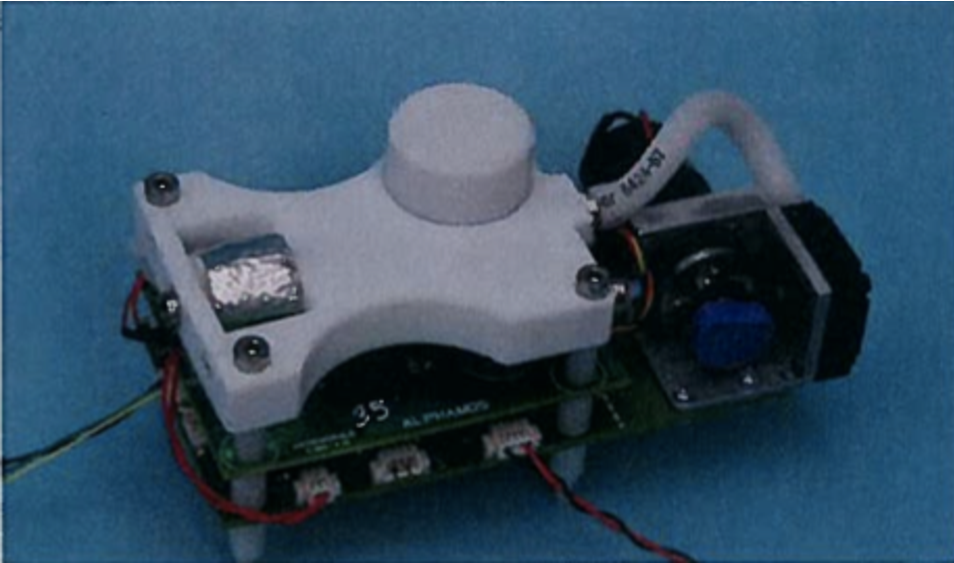
\includegraphics[width=4in]{img/sensor.pdf}
\caption{Alpha MOS NEEM chemical sensor.}
\label{fig:sensor}
\end{center}
\end{figure}

\label{sec:mount}

\subsubsection{Data Flow}

Data flow through the system is illustrated in Figure \ref{fig:acquisition}. The
chemical sensor passes concentration readings to the estimator at a rate of 1
Hz. When the estimator receives each new reading, it updates its model of the
chemical source's location, and passes the
parameters of this model to the planner. Using this estimate, the planner then
decides what direction the robot should move in and commands the robot to move.

\begin{figure}
\begin{center}
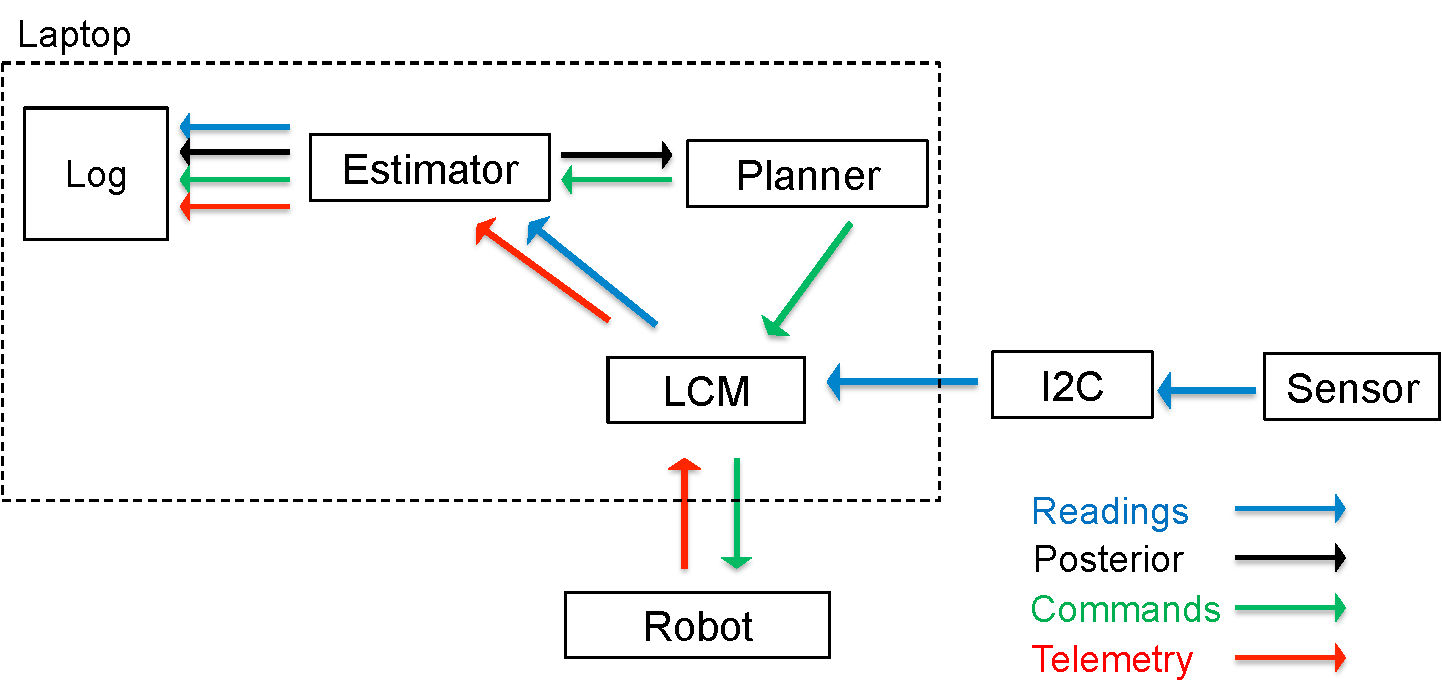
\includegraphics[width=6in]{img/acquisition.pdf}
\caption{The components of the system, and the paths along which data is
  communicated. Messages are passed among different components of the robot's
  software using the LCM protocol. All messages are issued at a rate of 1 Hz.
  Readings from the sensor include chemical concentration and hydrometry. The
  posterior distribution is the robot's current best estimate of the chemical
  source's location. Commands are sent in the form of a target position and
  orientation of the robot. Telemetry includes the robot's position, velocity,
  and attitude.}
\label{fig:acquisition}
\end{center}
\end{figure}

\subsubsection{Planner}

We will implement our two gradient descent planning algorithms as
follows: let $\hat{\vec{x_s}}$ be our current best estimate of the
source location, 
\begin{equation}
\hat{\vec{x_s}} = E[P(\vec{x_s}|c_1, \dots ,c_{n},\vec{x_r})]
\end{equation}
The simple gradient descent algorithm will move 0.5 meters in the
direction of the best source estimate $\hat{\vec{x_s}} - \vec{x_r}$.
The stochastic gradient descent algorithm will move in the direction
$\hat{\vec{x_s}} - \vec{x_r} + \vec{\epsilon}$, where $\vec{\epsilon}$
is a normally distributed random variable:
\begin{equation}
E[\vec{\epsilon}] = \vec{0} \qquad Cov[\vec{\epsilon}] = 
\left[\begin{array}{cc} \sigma^2 & 0 \\ 0 & \sigma^2 \end{array}\right]
\end{equation}
The robot will continually take measurements at a data rate of 1 Hz, issuing a
new command after receiving each reading.

\subsubsection{Estimator}

We will obtain the our best source location estimate through the
Bayesian inference technique of an Extended Kalman Filter (EKF)\cite{welch1995}. Given
a multivariate Gaussian prior distribution for the state, a command
given to the robot, and a measurement, the EKF will update this
probability distribution and return a multivariate Gaussian posterior
distribution for the state. The EKF deals with multivariate Gaussian
distributions characterized by a mean estimate for the state $\vec{\mu}$ and a
covariance matrix $\Sigma$. This probability distribution represents
our belief of the current state of the system. The state of the model depends only on the robot location $\vec{x_r}$ and the source location
$\vec{x_s}$, and so the state vector $\vec{x}$ is represented by:
\begin{equation} 
\vec{x} = \colvec{2}{\vec{x_r}}{\vec{x_s}}
\end{equation}
The mean estimate returned by the EKF is over the entire state vector,
nd we extract the component of the state that represents
the source location in order to get the best source location estimate $\vec{x_s}$
\begin{equation}
\vec{\mu} = \colvec{2}{\hat{\vec{x_r}}}{\hat{\vec{x_s}}}
\end{equation}
This best source location estimate can be passed to the planner, so
the planner can choose the next location to move to.

\subsection{Experimental Process}
\subsubsection{Test Environment}

Our experiment will be conducted in three closed rooms with irregular shapes.
The floorplans of the rooms are shown in Figure \ref{fig:floorplans}. The
ventilation systems of the room will be undisturbed in order to keep the test
environment close to that of a typical indoor environment. A sketch of the
experimental setup is shown in Figure~\ref{fig:layout}. Parameters of the
experiment are shown in Table \ref{tab:parameters}.

\begin{table}
\caption{Parameters of the experiment.}
\begin{center}
\begin{tabular}{|p{\tablewidthtwo}|p{\tablewidthtwo}|}
\hline
Chemical used as source & Liquid ethanol, 70\% \\ \hline
Surface area of chemical vapor source & 0.018 $\text{m}^2$\\ \hline
Vertical distance between sensor plane and
test room floor & 0.3 $\text{m}^2$ \\ \hline
Minimum initial distance between sensor and chemical & 2 $\text{m}$ \\ \hline
Radius of localization & 0.2 $\text{m}$ \\ \hline
Delay between robot start and source exposure & 30 minutes \\ \hline
\end{tabular}
\end{center}
\label{tab:parameters}
\end{table}

\begin{figure}
\begin{center}
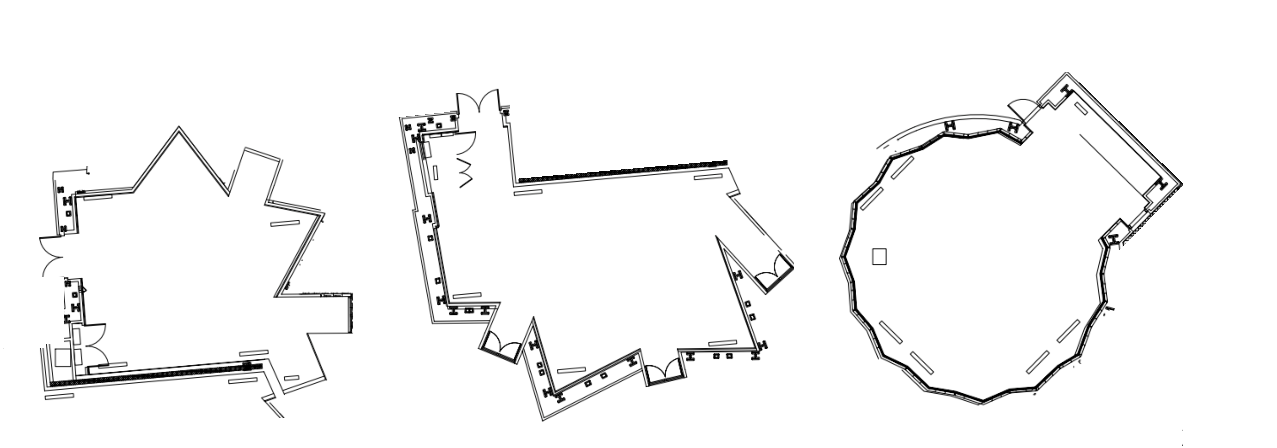
\includegraphics[width=7in]{img/rooms.pdf}
\caption{The rooms in the Stata Center where the experiments will
  be carried out.  From left to right, the room numbers are D461,
  D463, and G449.}
\label{fig:floorplans}
\end{center}
\end{figure}


\begin{figure}
\begin{center}
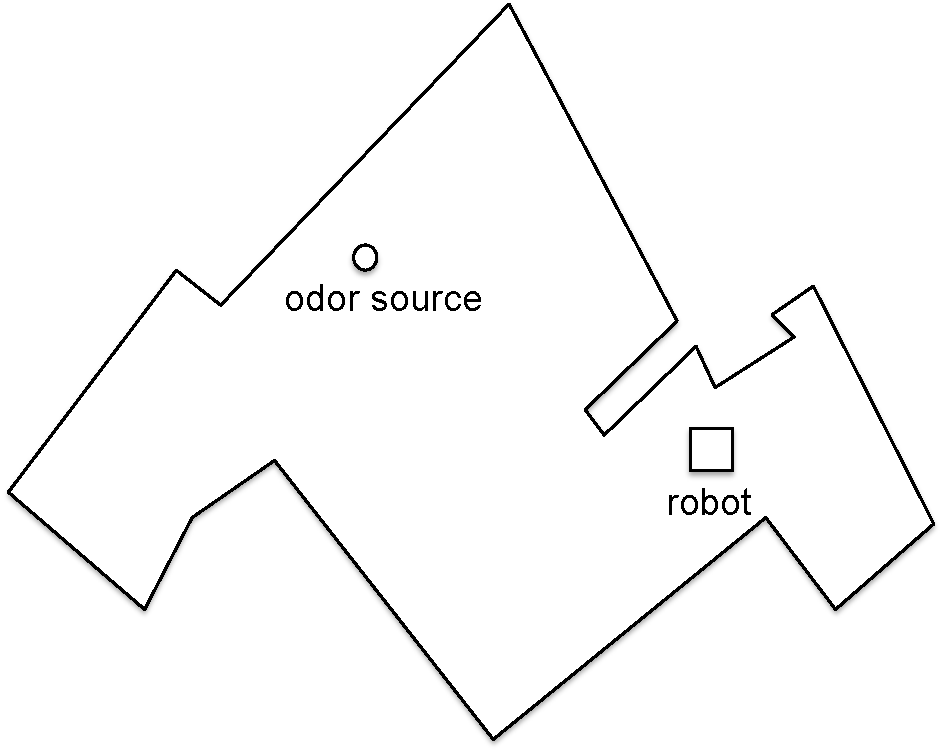
\includegraphics[width=3in]{img/layout.pdf}
\caption{Sketch of experimental setup.}
\label{fig:layout}
\end{center}
\end{figure}


\subsubsection{Test Procedure}

An exposed dish of ethanol will be placed at a random location in the test room
30 minutes before each trial begins, and will remain undisturbed at this
location for the entirety of the trial. The exposed surface area of ethanol will
also remain constant. The initial position of the robot will also be determined
randomly for each trial, subject to the constraint that it is no less than 2 m
from the dish of ethanol.  The robot will be started remotely after the 30
minute delay.

Each trial will be terminated after 60 minutes. Preliminary experiments will be
run to ensure the robot can locate the source in under 60 minutes in for the
majority of the preliminary trials for one of the algorithms. If 60 minutes is
not sufficient time for the robot to localize the source, the maximum trial time
length will be increased.

Consecutive trials conducted in the same room will be separated by at least 2
hours, during which no ethanol is exposed. Due to regulations regarding the air
cycle rate for an office building, we can conservatively say that the air in one
of our experiment rooms will be replaced at least 4 times per hour. This implies
that 2 hours after an emitting source has been removed from the room we can be
confident that the room is clean of ethanol traces.

15 trials will be run for each of the two planners being tested. The trials will
be divided among the three rooms. The test matrix for the experiment is
presented in Table~\ref{tab:test-matrix}. 

\begin{table}
\caption{Test Matrix} 
\begin{center}
\begin{tabular}{|c|c|c|c|c|}
\hline
\textbf{Planning Algorithm} &
\begin{tabular}{c}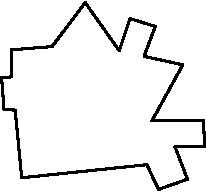
\includegraphics[width=\tablewidth]{img/D461.pdf} \\
D461 \end{tabular} &
\begin{tabular}{c}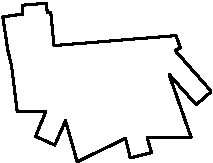
\includegraphics[width=\tablewidth]{img/D463.pdf} \\
D463 \end{tabular} &
\begin{tabular}{c}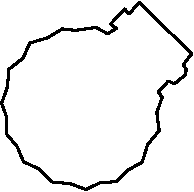
\includegraphics[width=\tablewidth]{img/G449.pdf} \\
G449 \end{tabular} \\ \hline
Simple Gradient Descent &  
\emph{mean time } & \emph{mean time } & \emph{mean time }\\\hline
Stochastic Gradient Descent & \emph{mean time } & \emph{mean time }  & \emph{mean time} \\ \hline
\end{tabular}
\end{center}
\label{tab:test-matrix}
\end{table}

\subsubsection{Data Acquisition}
At a rate of 1 Hz, the software platform will record and
timestamp all chemical sensor readings, robot position, planner commands, and
posterior estimates. The start time of the trial will be recorded
in the log file, and the mean and covariance of every posterior
distribution will be timestamped and recorded as well, the log files will hold all the
information necessary to extract localization time for each trial.
Given the mean and covariance of a multivariate Gaussian
posterior, by using a multivariate normal cumulative distribution
function we can calculate the percentage of the posterior probability
mass that falls within a circle of radius 0.2 m about the true source
location. We can then find the timestamp correlated with the first
posterior to have 90\% of its probability mass fall within 0.2 m of
the source location, and find the localization time for the trial by
subtracting the trial start time.

\section{Results}
\label{sec:results}
The results of this experiment contradict the hypothesis presented in
section \ref{sec:hos}.  This section contains  a summary of experimental data
and detailed statistical analysis of the data to assess the
hypothesis.

\subsection{Experimental Data}
For each of the nine source locations, table \ref{tab:data} shows the
ratio of the localization rate of
a trial using the stochastic planner to the localization rate of
a trial using the simple gradient descent (greedy) planner, as well as
the raw quantities used to calculate this ratio. $m_0$ is the initial sum of
the probabilities of particle filter particles located inside the 1
meter localization radius for each trial, and $m_f$ is the final sum
of the probabilities of the same particles. The localization rate of
each trial is calculated according to the equation $rate =
\frac{m_f/m_0}{T_{trial}}$ where $T_{trial}$ is the length of the
trial in minutes.  The ratio $R$ is given by the equation $R =
\frac{rate_{stoch}}{rate_{greedy}}$ and serves as a numerical
comparison between the localization rate using the greedy planner and
the localization rate using the stochastic planner for each source location.

\begin{table}[htb]
\begin{center}
\begin{tabular}{|c||c||c||c||c||c||c||c||c||c|}
\hline
 Source Location & 1 & 2 & 3 & 4 & 5 & 6 & 7 & 8 & 9 \\
\hline \hline
$m_{0_{greedy}}$ & 0.0502 & 0.0450 & 0.0500 & 0.0500 & 0.0497 & 0.0481 & 0.0493 & 0.0506 & 0.0497 \\
\hline
$m_{f_{greedy}}$ & 0.0468 & 0.0451 & 0.2935 & 0.0511 & 0.0519 & 0.0492 & 0.0562 & 0.0503 & 0.0518 \\
\hline
$r_{greedy}$ & 0.0259 & 0.0286 & 0.1656 & 0.0282 & 0.0298 & 0.0286 & 0.0303 & 0.0280 & 0.0293 \\
\hline
$m_{0_{stoch}}$ & 0.0502 & 0.0450 & 0.0500 & 0.0500 & 0.0497 & 0.0484 & 0.0493 & 0.0506 & 0.0490 \\
\hline
$m_{f_{stoch}}$ & 0.0521 & 0.0483 & 0.0525 & 0.0491 & 0.0480 & 0.0487 & 0.0495 & 0.0515 & 0.0491 \\
\hline
$r_{stoch}$ & 0.0295 & 0.0296 & 0.0299 & 0.0279 & 0.0268 & 0.0288 & 0.0280 & 0.0285 & 0.0280 \\
\hline
\hline
$R = \frac{rate_{stoch}}{rate_{greedy}}$  & 1.1371 & 1.0345 & 0.1807 & 0.9869 & 0.9014 & 1.0056 & 0.9251 & 1.0164 & 0.9564\\
\hline
\end{tabular}
\caption{Experimental Data \label{tab:data} }
\end{center}
\end{table}

The mean $R_{mean}$ of the ratios $R$ for the nine source locations is equal to
$R_{mean} = 0.905$ and was used to assess the hypotheis as false. The
90\% confidence interval on $R_{mean}$ is $(0.7313,1.0787)$.

\subsection{Statistical Hypothesis Assessment}
A one-sided Student's t-test with 8 degrees of freedom on alternative
hypothesis $R_{mean} > 1.2$ gave a t-statistic of $-3.1591$ with a
corresponding p-value of $0.9933$.  Thus, the probabilty of
obtaining a measured ratio greater than or equal to $R_{mean} = 0.905$
is $99.3\%$ under the null hypothesis ($R_{mean} = 1.2$), so the
alternative hypothesis $R_{mean} > 1.2$ must be rejected.  Figure
\ref{fig:killer} shows a graphical representation of the experimental
data and the rejected hypothesis.

\begin{figure}
\begin{center}
\fbox{
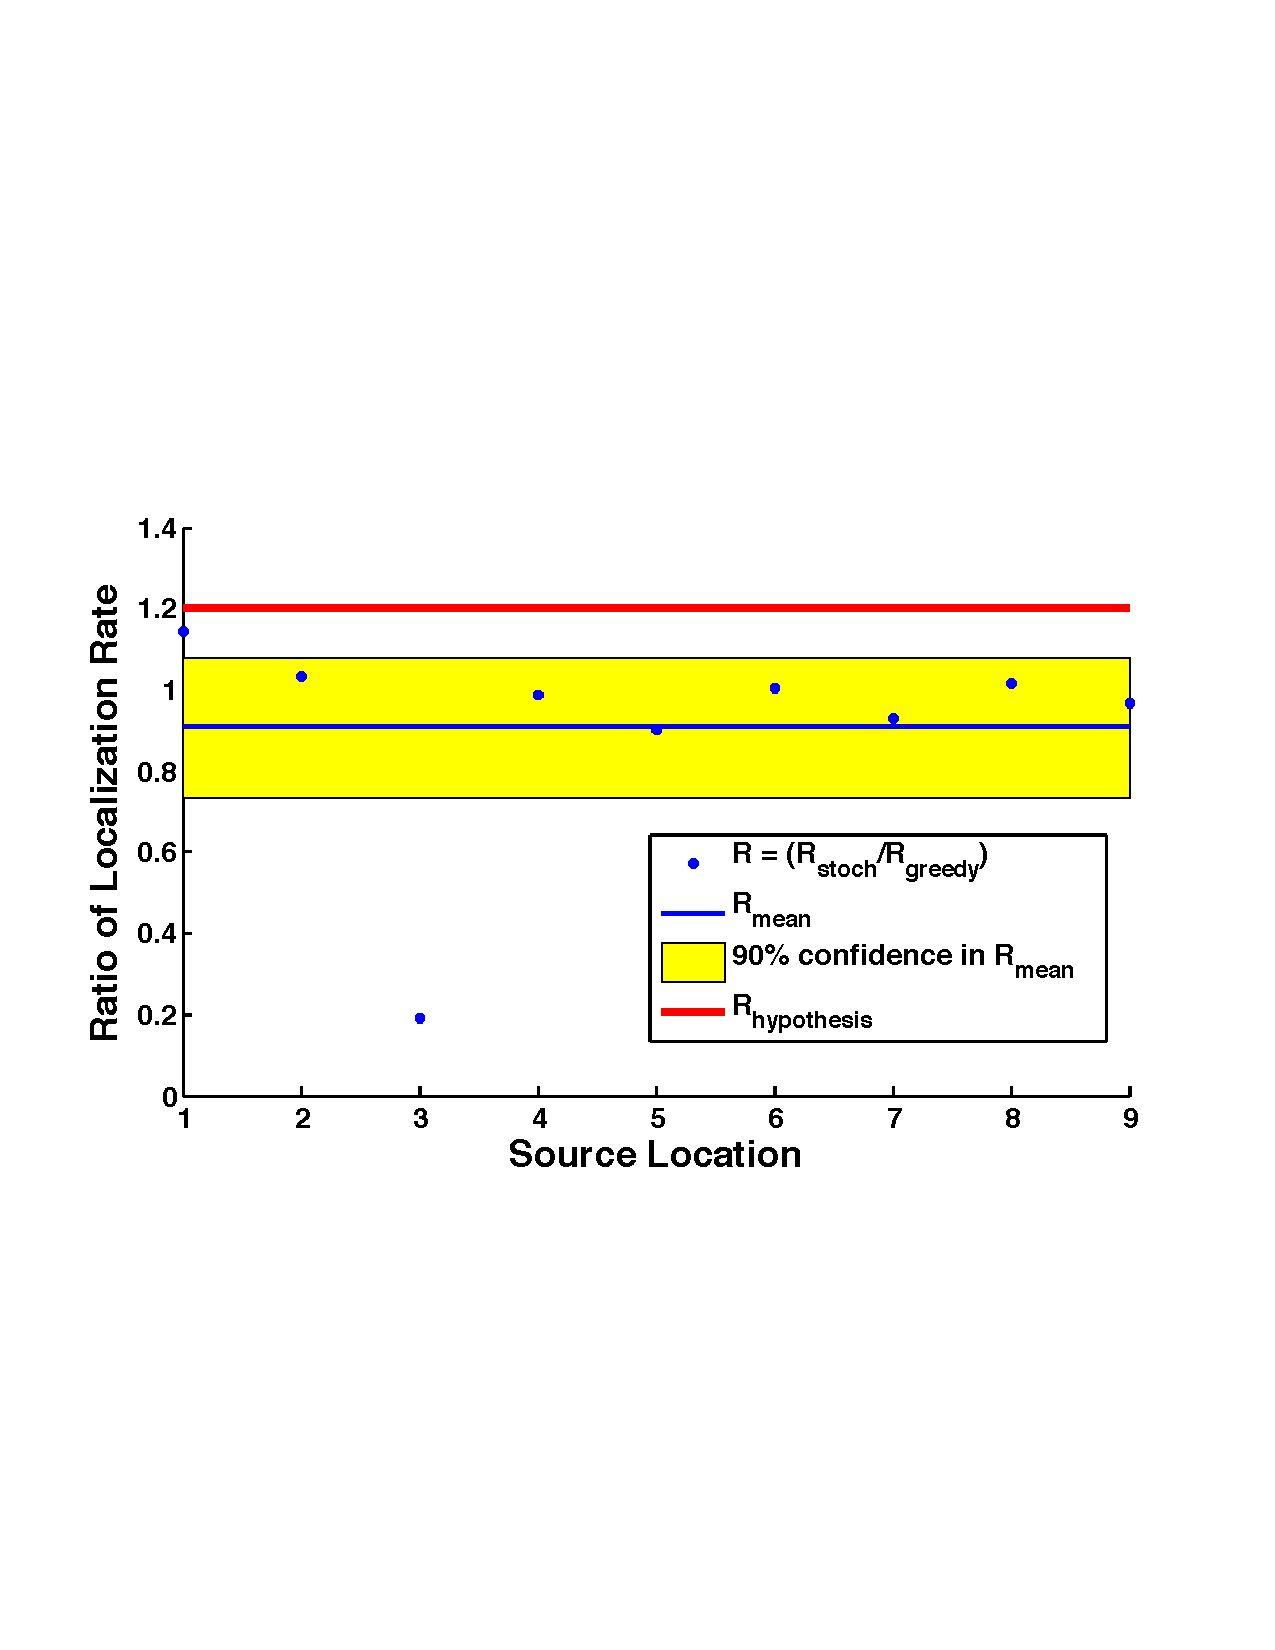
\includegraphics[width=6in]{img/Killer.pdf}}
\caption{Graphical representation of data and hypothesis.}
\label{fig:killer}
\end{center}
\end{figure}


\subsection{Additional Assessment of Results}
\label{sec:additional}
In addition to the assessment of the hypothesis, a two-sided Student's
t-test with 8 degrees of freedom was used on the hypothesis $R_{mean}
= 1$ to determine whether there was any statistically significant
difference in the mean localization rates.  This test gave
a t-statistic of $-1.0174$ and a p-value of $0.3388$, showing that
there is no statistically significant difference in the mean localization
rate achieved with the stochastic planner and the rate achieved with
the simple gradient descent planner.

\section{Discussion}
As described in the previous section, the stochastic planner was not
shown to produce a higher mean localization
rate than the simple gradient descent planner.  One possible cause may
have been
that the system did not produce a statistically significant increase
in the sum of probability mass inside the localization radius using
either planner.  The results of a two-sided Student's t-test on the
null hypothesis $\frac{m_f}{m_0} = 1$ are given in table
\ref{tab:nofind}.  Although the t-statistics show some increase in the
sum of probability mass inside the localization radius,
particularly in the case of the stochastic planner, this increase is
not significant at a 10\% level.

\begin{table}[htb]
\begin{center}
\begin{tabular}{|c||c|c|}
\hline
& t-statistic & p-value \\
\hline \hline
Greedy Planner & 1.0296 & 0.3333\\
\hline
Stochastic Planner& 1.3921 &0.2014\\
\hline
\end{tabular}
\caption{Students t-test for an increase in the sum of probability
  mass inside the localization radius over the time of a trial.
  These results show no statistically significant increase. \label{tab:nofind} }
\end{center}
\end{table}


One reason that the probability mass inside the localization
radius was not shown to increase over the time of a trial may have been
the presence of air currents in the room due to the ventilation
system, the motion of the robot, and other random disturbances. Currents may have invalidated the
assumption that the air directly above the true source location
holds a higher chemical vapor concentration than all surrounding
points.  A qualitative drifting behavior was observed in carrying out
the experiment, where higher concentration measurements were taken
at a distance of one to two meters in one direction from the source than were
taken at similar distances in other directions, and even at the exact
source location.  Further experimental characterization of indoor
chemical dispersion is necessary to confirm this drifting
behavior quantitatively.  The robotic localization system tested in
this experiment attempts to localize the area of highest
concentration, since the estimation algorithms assume the area of highest
concentration to be the location of the true source.  If the true
source location is in fact different from the location of the
highest chemical vapor concentration, the system may not be able to accurately
localize the source, regardless of which planner is used.  The
possibility of system failure in the manner described represents a lack of robust estimation techniques, and
calls for further research in the area of estimation algorithms for
indoor robotic odor localization.

The stochastic planner was expected to produce a greater localization
rate than the simple gradient descent planner due to the fact that it
was expected to gather concentration measurements from a larger
percentage of the test room area.  In experimental trials with the
stochastic planner, the system did gather measurements from a larger
area than in trials with the greedy planner.  This result is shown
qualitatively by the comparison of robot paths in figure \ref{fig:paths} and
quantitatively in table \ref{tab:paths}, where $A_{greedy}$ and
$A_{stoch}$ are the percentage of the area of the test room ``covered''
using the greedy planner and the stochastic planner respectively.  For
the purpose of this analysis, all of the area within 1 meter of the
location where any concentration measurement was taken during a trial
is considered to be ``covered'' in that trial.

\begin{figure}
\begin{center}
\fbox{
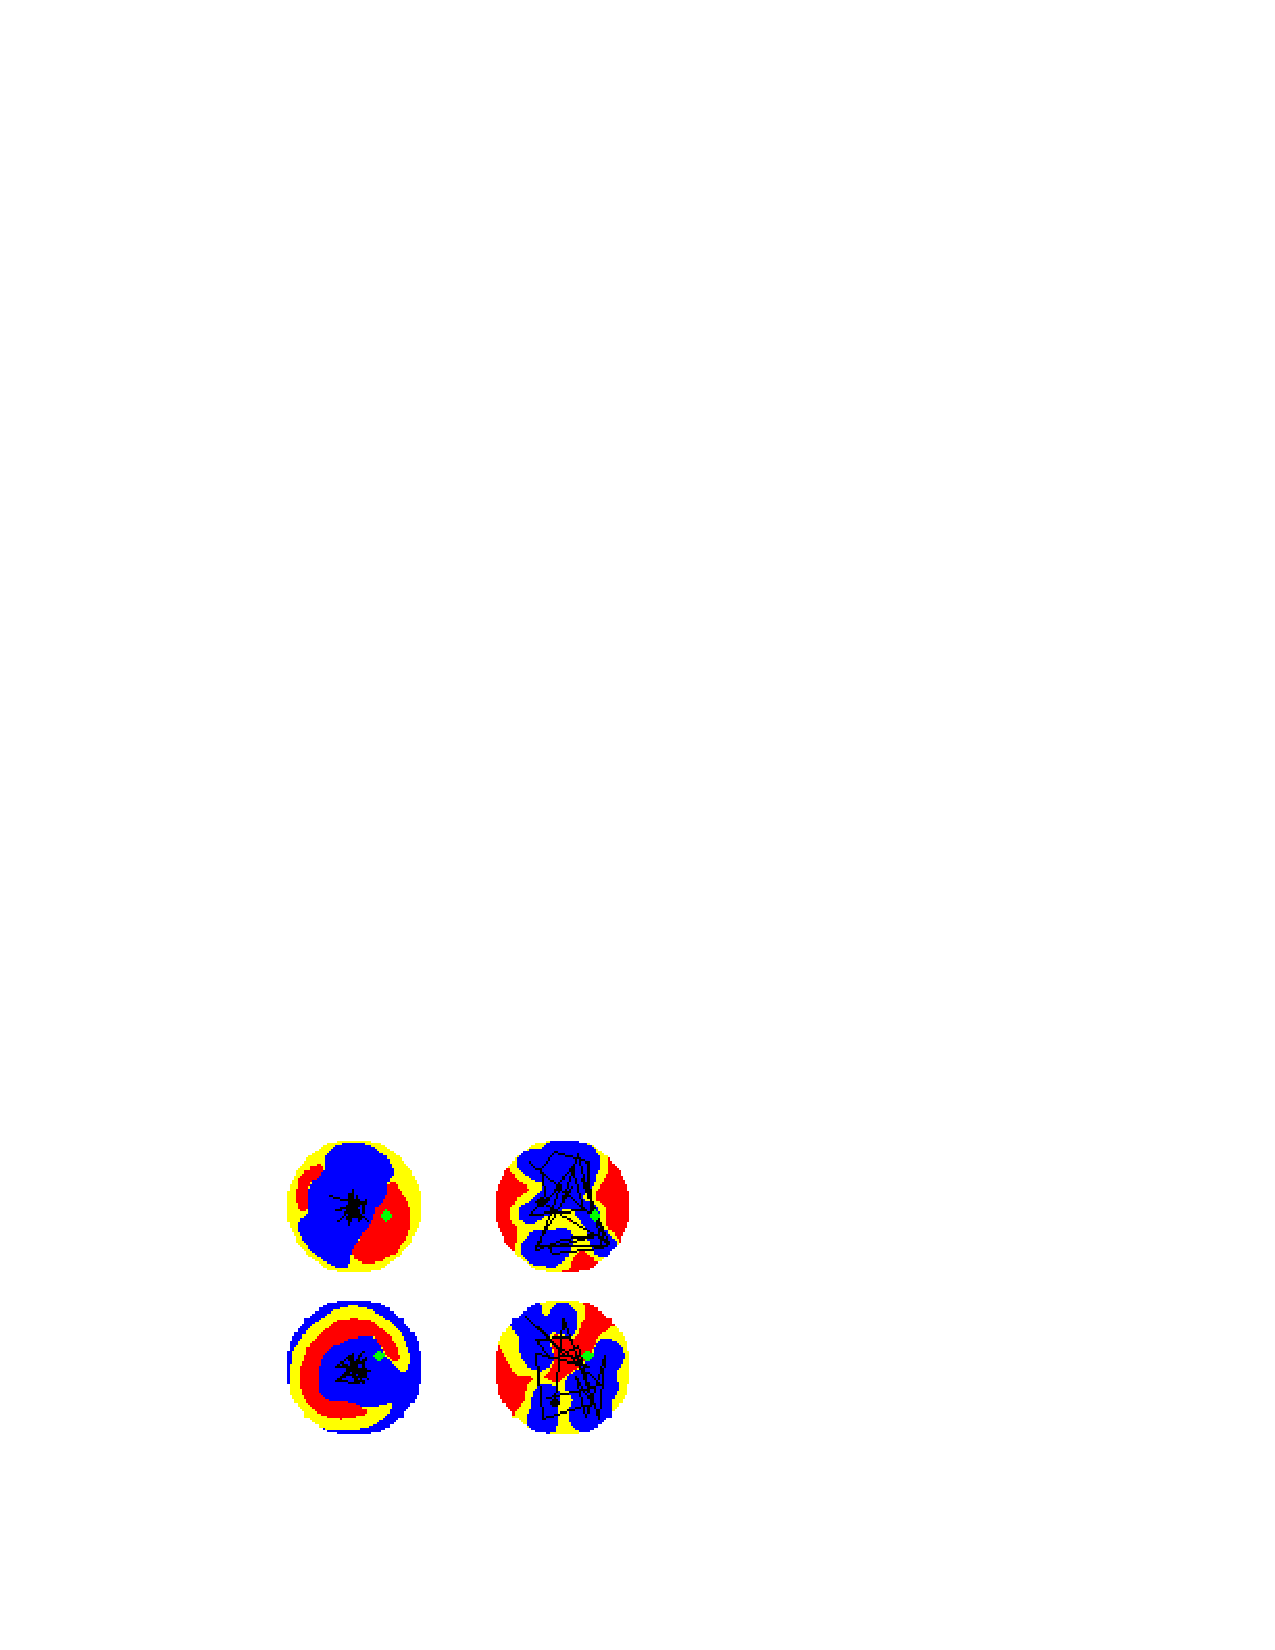
\includegraphics[width=6in]{img/paths.pdf}}
\caption{Comparison of robot paths and resulting final particle filter
  probability distributions using the greedy planner (left) and the
  stochastic planner (right) for source locations 7 (top) and 8 (bottom). The
  robot paths are shown in black, where each corner represents a
  measurement location, and the true source locations are
  shown in green.  The circular color fields represent the particle
  filter probability distributions.  The particles making up the top 25\% of the
  probability mass is shown in red, the particles making up the next
  25\% are shown in yellow, and the bottom 50\% are shown in blue. It
  is clear that the different planners produce different distributions
of measurements over the space in the test room, and this results in
different final particle filter probability distributions.}
\label{fig:paths}
\end{center}
\end{figure}

\begin{table}[htb]
\begin{center}
\begin{tabular}{|c||c||c||c||c||c||c||c||c||c|}
\hline
 Source Location & 1 & 2 & 3 & 4 & 5 & 6 & 7 & 8 & 9 \\
\hline \hline
$A_{greedy}$ & 0 & 0 & 0 & 0 & 0 & 0 & 0 & 0 & 0 \\
\hline
$A_{stoch}$ & 0 & 0 & 0 & 0 & 0 & 0 & 0 & 0 & 0 \\
\hline
\end{tabular}
\caption{Experimental Data \label{tab:paths} }
\end{center}
\end{table}

The differences in the distribution of measurement locations over the test room
produced by the greedy planner and the stochastic planner caused the
two planners
to produce different final particle filter probability distributions,
as illustrated qualitatively in figure \ref{tab:paths}.  However, as
discussed in section \ref{sec:results}, the difference in final
probability distributions did not produce a statistically significant
difference in the localization rate.  As discussed earlier in this
section, it is possible that the point of highest concentration is
not the true source location.  If this is the case, the use of a localization radius about
the true source location
to determine the localization rate may not fully assess the
relative performance of the two planners.  Though the use of a
localization radius accurately
assesses the performance of the system in localizing the true source,
and thus correctly and accurately assesses the hypothesis, this metric only takes
into account a subset of the information gained by the particle filter
during a trial.

It is feasible that a more robust estimaton technique could be developed through
future research that takes into account any differences that may exist
between the true source location and the location of highest chemical
vapor concentration.  To gain preliminary intuition regarding the
relative performance of the simple gradient descent planner and the
stochastic planner in such a circumstance, it was desired to know
whether there was any difference between the full amount of information
gained in a trial using the greedy planner, and the amount gained
using a stochastic planner.  The amount of information gained in each
trial was measured by calculating the Kullback – Leibler divergence (KL
divergence) of
the final particle filter probability distribution from the initial
uniform distribution where all of the particles are assigned the same
probability.  The KL divergence of the particle filter probability
distribution in each trial is shown in table \ref{tab:allinfo}.

\begin{table}[htb]
\begin{center}
\begin{tabular}{|c||c||c||c||c||c||c||c||c||c|}
\hline
 Source Location & 1 & 2 & 3 & 4 & 5 & 6 & 7 & 8 & 9 \\
\hline \hline
Greedy KL divergence & 0 & 0 & 0 & 0 & 0 & 0 & 0 & 0 & 0 \\
\hline
Stochastic KL divergence & 0 & 0 & 0 & 0 & 0 & 0 & 0 & 0 & 0 \\
\hline
Ratio $\frac{KL_{stoch}}{KL_{greedy}}$ & 0 & 0 & 0 & 0 & 0 & 0 & 0 & 0 & 0 \\
\hline
\end{tabular}
\caption{Kullback-Leibler divergence of the final particle filter
  probability distribution from the initial uniform particle
  probability distribution.  This is a measure of how much
  information about the environment was gained by the system in each trial. \label{tab:allinfo} }
\end{center}
\end{table}

The mean of the ratios $\frac{KL_{stoch}}{KL_{greedy}}$ over the 9
source locations is equal to $mean(\frac{KL_{stoch}}{KL_{greedy}}) =
TROYFILLTHISIN$.  A two-sided Student's t-test with the null hypothesis
$mean(\frac{KL_{stoch}}{KL_{greedy}}) = 1$ gave a t-statistic of
$-0.3851$ and a p-value of $0.7102$.  This 



\section{Summary and Conclusion}

\section{Acknowledgments}

\newpage
\bibliographystyle{aiaa}
\bibliography{sources}
\nocite{*}

\end{document}